\documentclass{beamer}

%% Tema y configuraciones (misma anatomía de mis otros cursos)
\usetheme{Boadilla}
\usecolortheme{default}
\setbeamertemplate{navigation symbols}{}
\usepackage[utf8]{inputenc}
\usepackage[T1]{fontenc}
\usepackage{xcolor}
\usepackage{graphicx}
\usepackage{booktabs}
\usepackage{array}
\usepackage{colortbl}
\hypersetup{
    colorlinks=true,
    linkcolor=.,
    urlcolor=blue,
    citecolor=.,
}

%% Colores de apoyo (los mismos de la semana 5)
\definecolor{verdeok}{RGB}{39,124,74}
\definecolor{rojoal}{RGB}{198,40,40}
\definecolor{naranjal}{RGB}{230,126,34}
\definecolor{grisclaro}{RGB}{242,243,246}
\definecolor{azulcaso}{RGB}{28,60,120}

%% Encabezado
\title[06327-ECO]{Analítica para los negocios \\ 06327-ECO}
\subtitle{Semana 13: Los segmentos de Cóndor --- ¿quiénes son y dónde está la plata en riesgo?}
\author{Eduard F. Martínez González, Ph.D.}
\institute[]{Departamento de Economía, Universidad Icesi}
\date{\textcolor{rojoal}{[fecha por definir]}}

%%=================================================
\begin{document}

\begin{frame}
\titlepage
\end{frame}

%%=================================================
\begin{frame}{Objetivo de la sesión}
\small
Hoy se acaba la hoja de respuestas: se agrupan los mismos 8.000 clientes de Cóndor \textbf{sin target}, y los grupos se defienden con perfilamiento.

\vspace{0.15cm}
\begin{itemize} \setlength{\itemsep}{0.16cm}
  \item Recencia, frecuencia y monto: el bloque RFM de la base.
  \item Qué pasa cuando no se escala, y cómo se elige el número de segmentos cuando las métricas no votan lo mismo.
  \item El cruce con lo construido en las semanas 11 y 12: el riesgo y el valor en riesgo.
\end{itemize}

\vspace{0.15cm}
\begin{block}{La idea que gobierna la sesión}
Un segmento solo sirve si se puede \textbf{nombrar} y \textbf{accionar}. Y la acción se decide mirando dos cosas a la vez: cuánto riesgo hay y cuánta plata está en juego.
\end{block}
\end{frame}

%%=================================================
\begin{frame}{¿Dónde estamos en el curso?}
\small
\begin{itemize} \setlength{\itemsep}{0.16cm}
  \item \textbf{Semana 6:} el EDA --- quiénes abandonan.
  \item \textbf{Semana 10:} el juicio --- el sobre sellado y la tabla del líder.
  \item \textbf{Semana 11:} quién se va --- el bosque empata con la regla del EDA y compra la perilla: un riesgo para cada cliente.
  \item \textbf{Semana 12:} cuánto gasta --- la regla de Finanzas es casi imposible de mejorar; el valor en riesgo junta las dos preguntas.
  \item \textbf{Semana 13 (hoy):} quiénes son --- segmentos sin target, cruzados con el riesgo y el valor.
\end{itemize}
\end{frame}

\begin{frame}[noframenumbering]{Roadmap}
\tableofcontents
\end{frame}

%%=================================================
\section{Las variables y la escala}

\begin{frame}[noframenumbering]{Roadmap}
\tableofcontents[currentsection]
\end{frame}

\begin{frame}{La pregunta de hoy}
\small
\begin{block}{Marketing y Growth}
``Queremos segmentos de clientes con personalidad, para diseñar una acción distinta para cada uno. Y queremos saber en cuál de ellos está la plata en riesgo.''
\end{block}

\vspace{0.15cm}
\begin{itemize} \setlength{\itemsep}{0.12cm}
  \item \textbf{Tarea:} segmentación --- agrupar sin target. Nadie dice de antemano cuántos grupos hay ni cuáles son.
  \item \textbf{Variables:} recencia, frecuencia y monto (RFM). Quedan fuera \texttt{abandono} --- se guarda para ver si los segmentos lo separan sin haberlo visto --- y \texttt{gasto\_proximo\_trim}, del futuro.
  \item \textbf{Método:} k-means, que agrupa por distancia alrededor de centroides.
\end{itemize}
\end{frame}

\begin{frame}{Paso 1 · ¿Con qué variables se segmenta?}
\small
\begin{columns}[T]
\column{0.5\textwidth}
\centering
\footnotesize
\begin{tabular}{lr}
\toprule
Variable & Desviación \\
\midrule
Recencia (días) & 63,4 \\
Frecuencia (transacciones) & 21,0 \\
Monto total (pesos) & 623.353,1 \\
\bottomrule
\end{tabular}
\column{0.48\textwidth}
\begin{itemize} \setlength{\itemsep}{0.12cm}
  \item k-means mide distancias: cada variable pesa según su escala.
  \item El monto varía unas \textbf{10.000 veces} más que la recencia y \textbf{30.000} más que la frecuencia.
\end{itemize}
\end{columns}
\pause
\vspace{0.3cm}
\begin{alertblock}{Hallazgo 1}
Una variable no es como las otras. Si nadie la pone en su lugar, la distancia será, en la práctica, solo monto.
\end{alertblock}
\end{frame}

\begin{frame}{Paso 2 · ¿Qué pasa si no se escala?}
\small
\begin{columns}[T]
\column{0.58\textwidth}
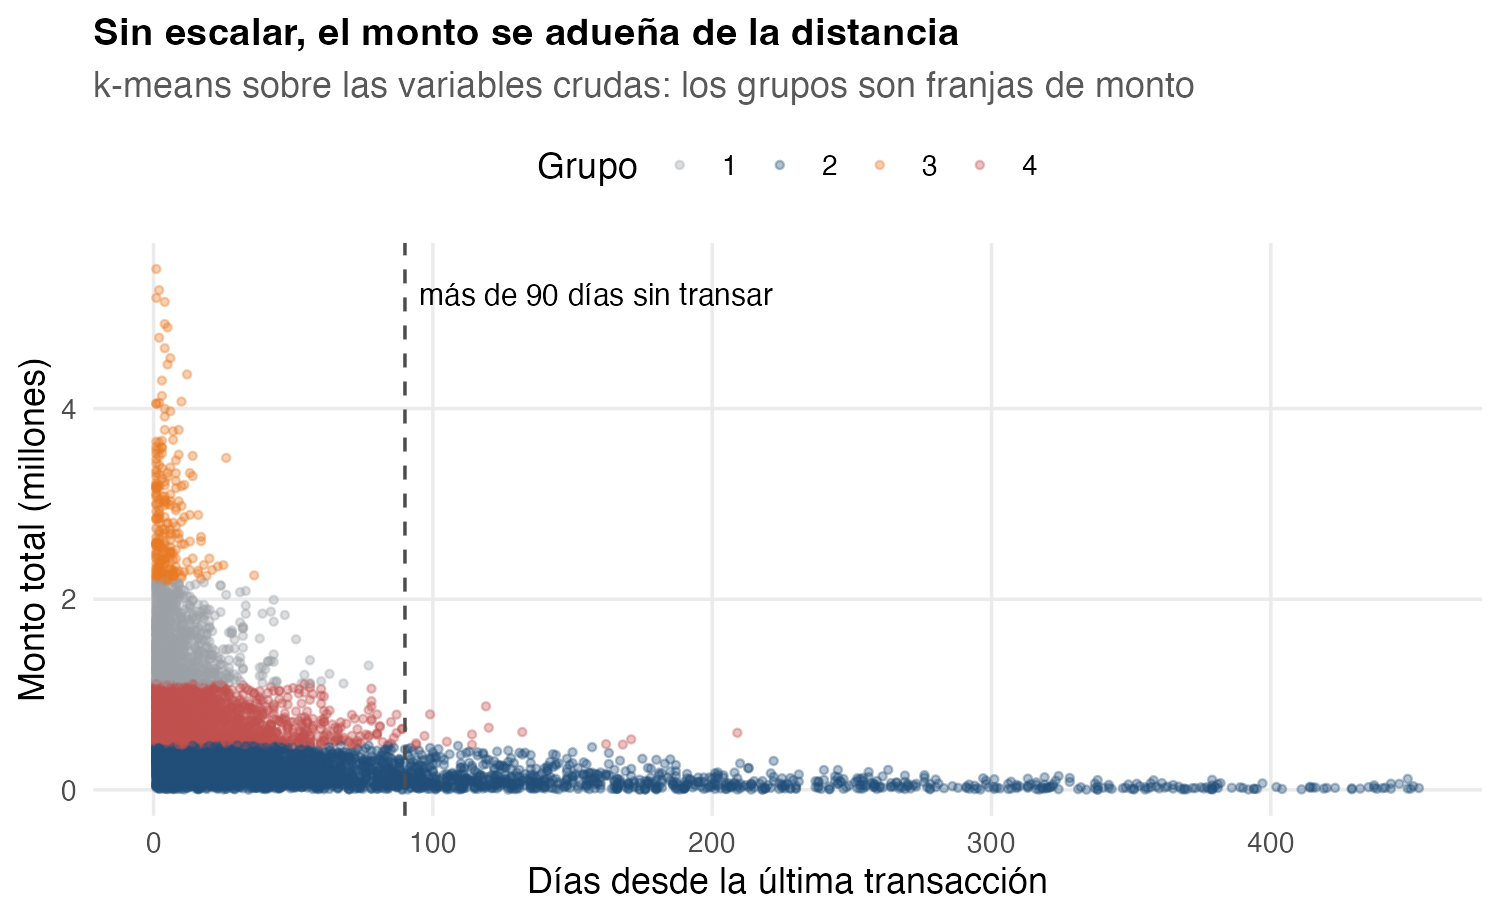
\includegraphics[width=\textwidth]{pic/fig_s13_crudo.png}
\column{0.4\textwidth}
\footnotesize
k-means con $k = 4$ sobre las variables crudas:
\begin{itemize} \setlength{\itemsep}{0.06cm}
  \item Montos medianos de \textbf{202.500}, \textbf{700.900}, \textbf{1.442.800} y \textbf{2.656.750}: franjas de plata.
  \item De los \textbf{886} clientes con más de 90 días sin transar, \textbf{872} quedan en el grupo más grande (4.358 clientes, recencia mediana de 30 días).
\end{itemize}
\end{columns}
\pause
\vspace{0.1cm}
\begin{alertblock}{Hallazgo 2}
La distancia la secuestró el monto. Los clientes dormidos --- el grupo de mayor riesgo de la semana 6 --- \textbf{no aparecen por ningún lado}: quedaron diluidos en una franja de plata.
\end{alertblock}
\end{frame}

\begin{frame}{Paso 3 · ¿Cómo se pone a todos en la misma cancha?}
\small
\begin{itemize} \setlength{\itemsep}{0.2cm}
  \item Se \textbf{escala} cada variable: $z = (x - \bar{x}) / s$. A cada una se le resta su media y se divide por su desviación.
  \item Resultado: medias \textbf{0, 0, 0} y desviaciones \textbf{1, 1, 1} --- las tres pesan igual en la distancia.
  \item Un día sin transar y una transacción de más ahora pesan lo mismo que la diferencia típica de monto.
\end{itemize}
\vspace{0.2cm}
\begin{block}{La decisión del paso}
Siempre se escala antes de k-means. Y el perfil de los segmentos se lee después con los datos \textbf{originales}, en las unidades que entiende el negocio.
\end{block}
\end{frame}

%%=================================================
\section{Cuántos y quiénes}

\begin{frame}[noframenumbering]{Roadmap}
\tableofcontents[currentsection]
\end{frame}

\begin{frame}{Paso 4 · ¿Cuántos segmentos?}
\small
\begin{columns}[T]
\column{0.5\textwidth}
\centering
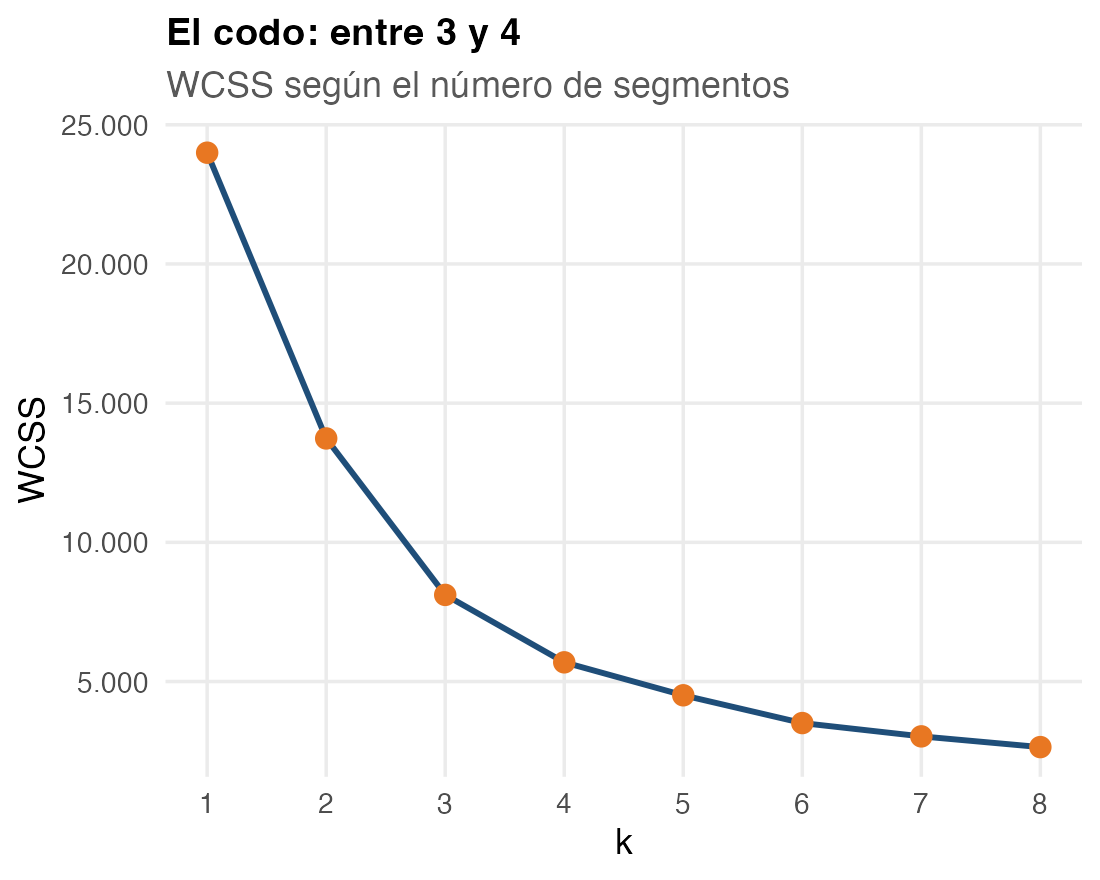
\includegraphics[width=0.78\textwidth]{pic/fig_s13_codo.png}
\column{0.5\textwidth}
\centering
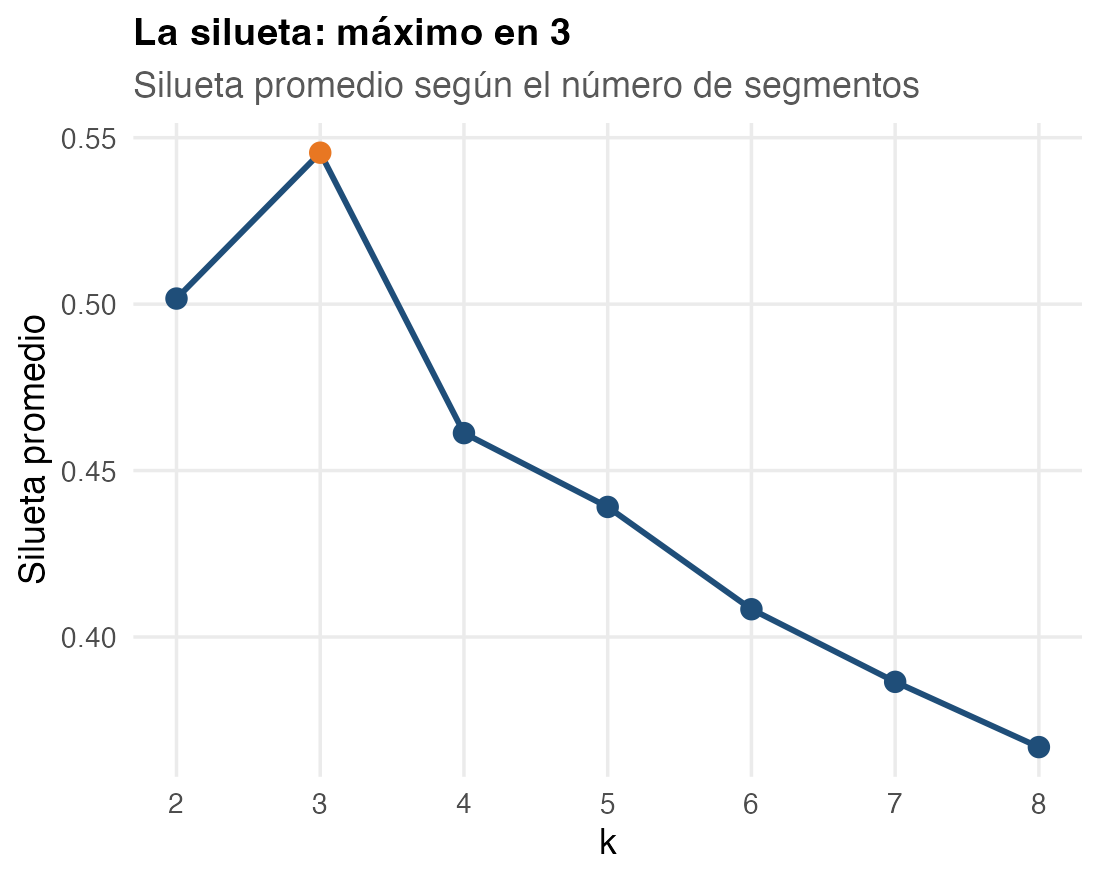
\includegraphics[width=0.78\textwidth]{pic/fig_s13_silueta.png}
\end{columns}
\vspace{-0.05cm}
\footnotesize
\begin{itemize} \itemsep1pt
  \item \textbf{Codo:} el tercer segmento compra $-$5.620 de compactación; el cuarto, $-$2.422; el quinto, apenas $-$1.184.
  \item \textbf{Silueta:} 0,502 · \textbf{0,545} · 0,461 · 0,439\ldots --- máximo en $k = 3$.
\end{itemize}
\pause
\begin{alertblock}{Hallazgo 4}
Las métricas no votan lo mismo. La regla práctica: \textbf{perfilar ambos}. Con $k = 4$ aparecen 549 clientes con más del doble de monto que los activos, que merecen una acción propia. $k = 4$ es más accionable.
\end{alertblock}
\end{frame}

\begin{frame}{Paso 5 · ¿Quiénes son?}
\small
\begin{columns}[T]
\column{0.5\textwidth}
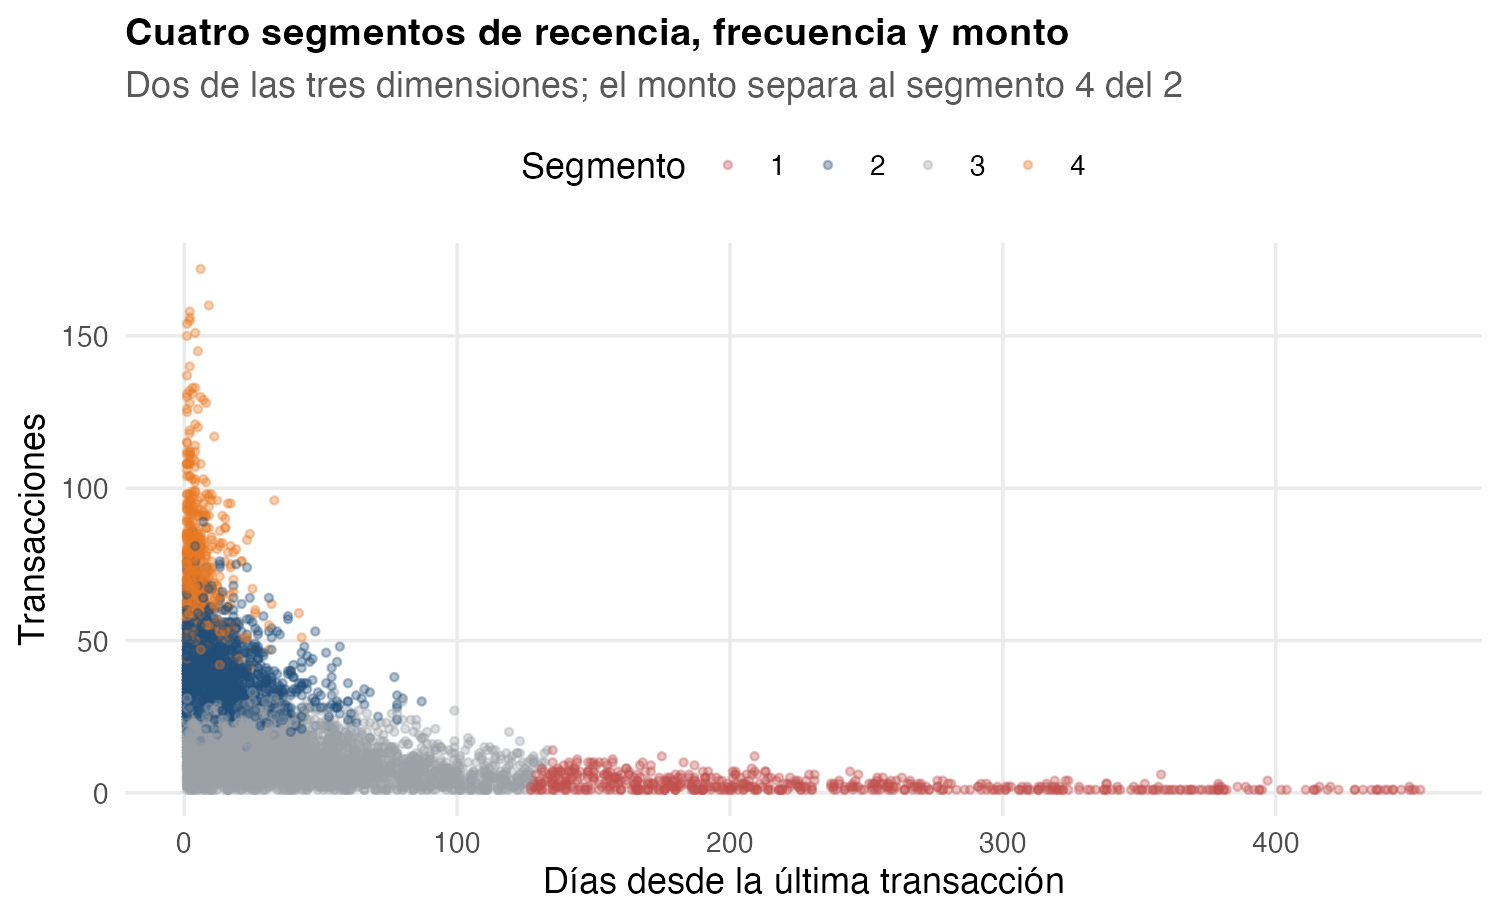
\includegraphics[width=\textwidth]{pic/fig_s13_segmentos.png}
\column{0.5\textwidth}
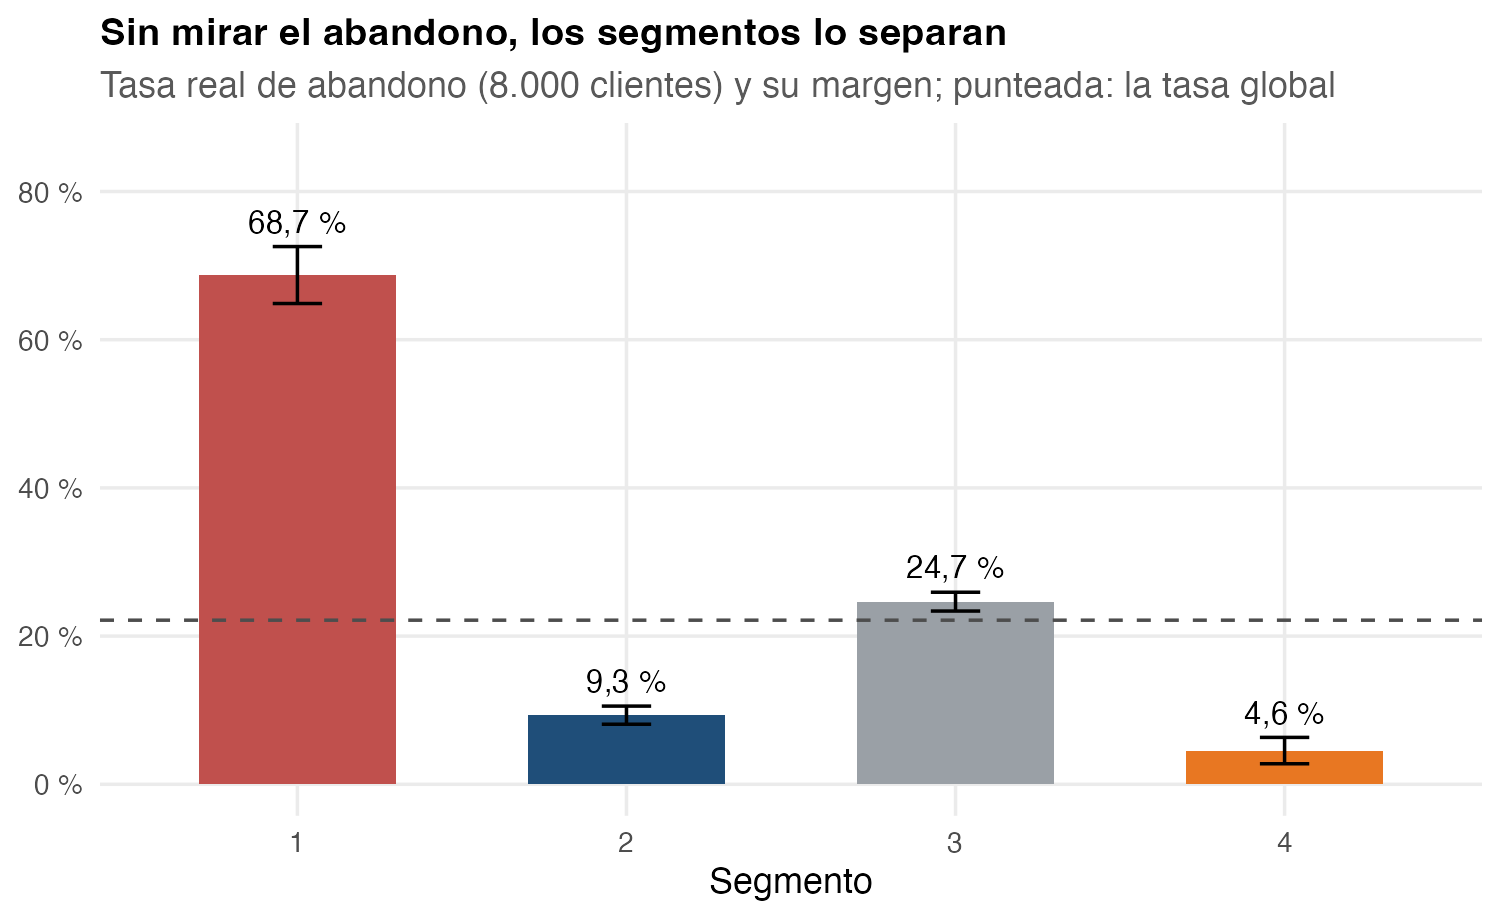
\includegraphics[width=\textwidth]{pic/fig_s13_abandono.png}
\end{columns}
\vspace{0.05cm}
\centering
\scriptsize
\begin{tabular}{crrrrc}
\toprule
Segmento & Clientes & Recencia & Frecuencia & Monto & Abandono \\
\midrule
1 & 582 & 204 días & 2 & 54.850 & 68,7 ± 3,8\,\% \\
2 & 2.261 & 7 días & 36 & 928.800 & 9,3 ± 1,2\,\% \\
3 & 4.608 & 22 días & 12 & 276.850 & 24,7 ± 1,3\,\% \\
4 & 549 & 4 días & 72 & 2.094.800 & 4,6 ± 1,8\,\% \\
\bottomrule
\end{tabular}
\raggedright
\small
\pause
\begin{alertblock}{Hallazgo 5}
Los segmentos se armaron \textbf{sin mirar el abandono}, y lo separan: del 68,7\,\% al 4,6\,\%, muy por encima de los márgenes.
\end{alertblock}
\end{frame}

%%=================================================
\section{La plata en riesgo}

\begin{frame}[noframenumbering]{Roadmap}
\tableofcontents[currentsection]
\end{frame}

\begin{frame}{Paso 6 · ¿Dónde está la plata en riesgo?}
\small
\begin{columns}[T]
\column{0.58\textwidth}
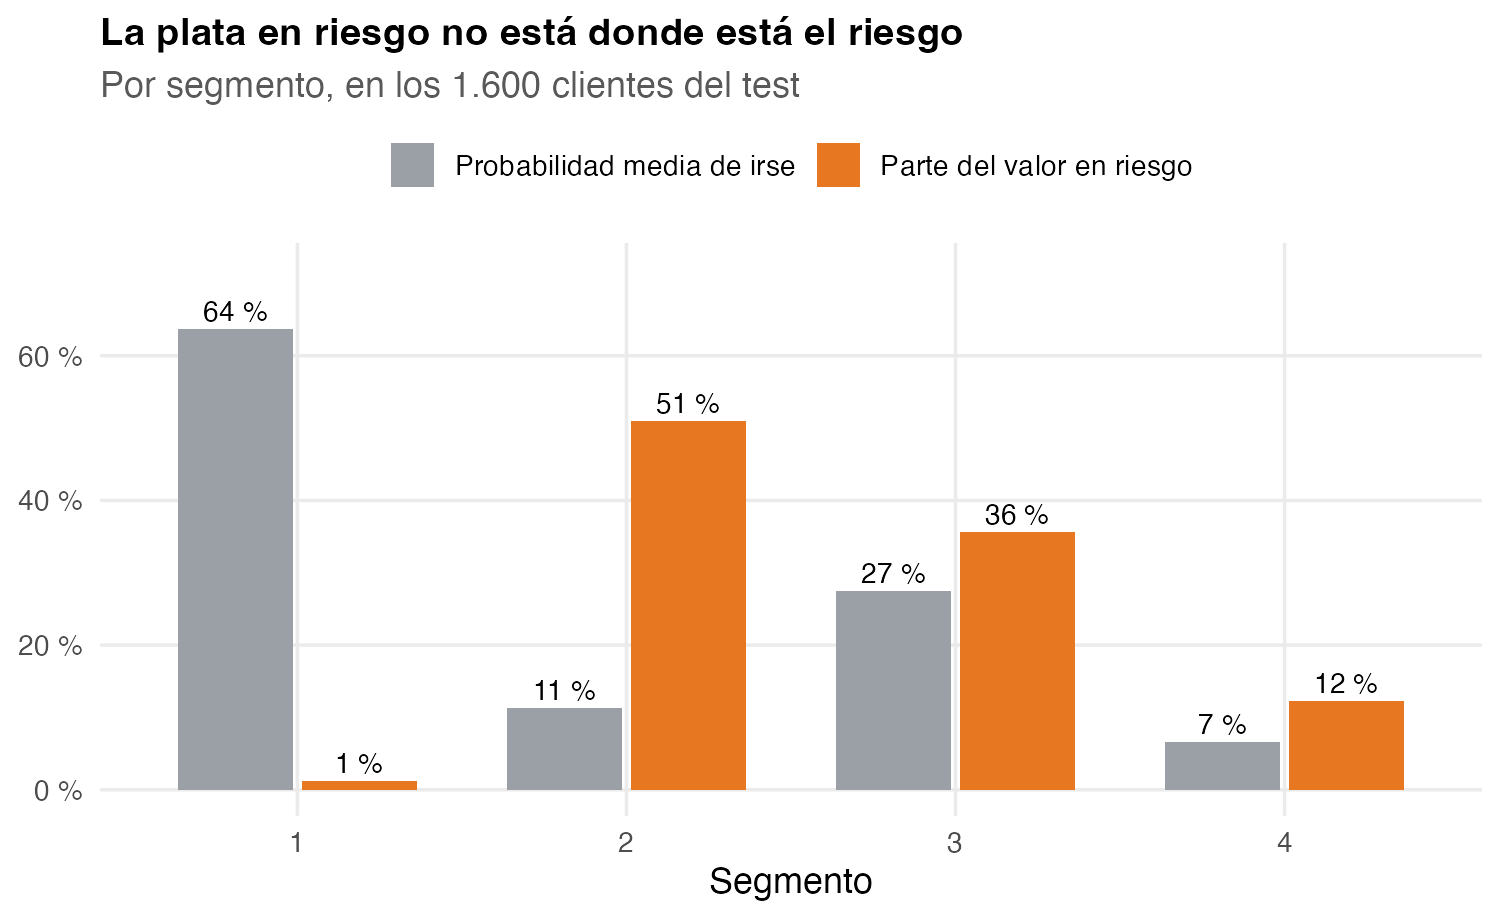
\includegraphics[width=\textwidth]{pic/fig_s13_valor.png}
\column{0.4\textwidth}
\footnotesize
\textbf{Valor en riesgo} = probabilidad de irse (semana 11) × gasto esperado (semana 12), en los 1.600 clientes del sobre.
\begin{itemize} \setlength{\itemsep}{0.06cm}
  \item Segmento 1: riesgo \textbf{0,637}; \textbf{1,2\,\%} del valor en riesgo.
  \item Segmento 2: riesgo \textbf{0,113}; \textbf{51\,\%} del valor en riesgo.
\end{itemize}
\end{columns}
\pause
\vspace{0.1cm}
\begin{alertblock}{Hallazgo 6 --- la lección de la semana}
\textbf{La plata en riesgo no está donde está el riesgo.} Una campaña que solo mire la probabilidad de irse llamaría a quienes menos plata ponen en juego.
\end{alertblock}
\end{frame}

%%=================================================
\section{Lo que queda}

\begin{frame}[noframenumbering]{Roadmap}
\tableofcontents[currentsection]
\end{frame}

\begin{frame}{El mapa de los segmentos}
\small
\centering
\footnotesize
\begin{tabular}{crrcc}
\toprule
Segmento & Clientes & Monto mediano & Abandono real & Parte del valor en riesgo \\
\midrule
1 & 582 & 54.850 & 68,7\,\% & 1,2\,\% \\
2 & 2.261 & 928.800 & 9,3\,\% & 51,0\,\% \\
3 & 4.608 & 276.850 & 24,7\,\% & 35,6\,\% \\
4 & 549 & 2.094.800 & 4,6\,\% & 12,2\,\% \\
\bottomrule
\end{tabular}

\raggedright
\small
\pause
\vspace{0.3cm}
\begin{block}{La decisión}
Una acción por segmento: reactivación barata y automática donde el riesgo es alto pero la plata poca; retención personalizada donde está la mitad del valor; un ejecutivo de cuenta para los de más monto --- el tratamiento aparte de la semana 12.
\end{block}
\end{frame}

\begin{frame}{Qué produce una segmentación --- y qué no}
\small
\begin{columns}[T]
\column{0.48\textwidth}
\textbf{Produce}
\begin{itemize} \setlength{\itemsep}{0.1cm}
  \item Grupos que se pueden nombrar y accionar.
  \item Un lenguaje común para Marketing, Growth y Finanzas.
  \item El mapa completo: quiénes son, cuánto riesgo tienen y cuánta plata ponen en juego.
\end{itemize}
\column{0.48\textwidth}
\textbf{No produce}
\begin{itemize} \setlength{\itemsep}{0.1cm}
  \item Una respuesta correcta: sin target, el analista valida con el perfil y la acción.
  \item Estabilidad garantizada: otro mes de datos puede mover los grupos.
  \item Causas: el segmento describe; no dice por qué un cliente se va.
\end{itemize}
\end{columns}
\end{frame}

\end{document}
